% NeuroSym: Neural-Symbolic SMT Solver — 2-Page Evaluation Report
% Compile with: pdflatex NeuroSym_Report.tex

\documentclass[10pt,twocolumn]{article}

\usepackage[margin=1.8cm,top=1.6cm,bottom=1.6cm]{geometry}
\usepackage{booktabs}
\usepackage{amsmath}
\usepackage{amssymb}
\usepackage{graphicx}
\usepackage{xcolor}
\usepackage{hyperref}
\usepackage{microtype}
\usepackage{enumitem}
\usepackage{titlesec}
\usepackage{fancyhdr}
\usepackage{tikz}
\usepackage{array}
\usepackage{multirow}
% Colors
\definecolor{gancolor}{RGB}{0,102,204}
\definecolor{satcolor}{RGB}{0,153,76}
\definecolor{unsatcolor}{RGB}{204,0,0}
\definecolor{rowgray}{RGB}{245,245,245}

% Section formatting
\titleformat{\section}{\normalsize\bfseries\color{gancolor}}{}{0em}{}[\titlerule]
\titleformat{\subsection}{\small\bfseries}{}{0em}{}
\titlespacing{\section}{0pt}{6pt}{3pt}
\titlespacing{\subsection}{0pt}{4pt}{2pt}

% Compact lists
\setlist[itemize]{noitemsep, topsep=2pt, leftmargin=*}

% Header/footer
\pagestyle{fancy}
\fancyhf{}
\renewcommand{\headrulewidth}{0.4pt}
\fancyhead[L]{\small\textit{NeuroSym — SMT-COMP 2026}}
\fancyhead[R]{\small\textit{NIT Warangal / University of Manchester}}
\fancyfoot[C]{\small\thepage}

\hypersetup{colorlinks=true, linkcolor=gancolor, urlcolor=gancolor, citecolor=gancolor}

% ─────────────────────────────────────────────────────────────────────────────
\begin{document}
% ─────────────────────────────────────────────────────────────────────────────

\twocolumn[{%
\begin{center}
  {\Large\bfseries NeuroSym: A Neural-Symbolic SMT Solver}\\[4pt]
  {\large\bfseries Evaluation Report — SMT-COMP 2026}\\[6pt]
  {\small
    Vishal Kumar Swain$^{1}$,\;
    Sangharatna Godboley$^{1}$,\;
    P.\ Radha Krishna$^{1}$,\;
    Avijit Das$^{2}$,\;
    Lucas Cordeiro$^{3}$
  }\\[2pt]
  {\footnotesize
    $^{1}$NIT Warangal \quad
    $^{2}$DRDO, LRDE Bengaluru \quad
    $^{3}$The University of Manchester
  }\\[2pt]
  {\footnotesize
    \texttt{vk25csr1p07@student.nitw.ac.in},\;
    \texttt{sanghu@nitw.ac.in},\;
    \texttt{prkrishna@nitw.ac.in},\;
    \texttt{avijitdas.lrde@gov.in},\;
    \texttt{lucas.cordeiro@manchester.ac.uk}
  }
\end{center}
\vspace{6pt}
\hrule
\vspace{8pt}
}]

% ─── ABSTRACT ────────────────────────────────────────────────────────────────
\noindent
\textbf{Abstract.}
NeuroSym is the \textbf{first GAN-guided solver} submitted to SMT-COMP.
It pairs an Iterative Refinement GAN (8 candidates per formula) with a
single symbolic fallback per theory: Bitwuzla for QF\_BV/QF\_ABV and
Z3 for QF\_LIA.
On 100 SMT-COMP 2025 QF\_BV benchmarks (5\,s timeout),
NeuroSym achieves a PAR-2 score of \textbf{949.0\,ms} — only 10\,ms
behind Bitwuzla (2024 winner, 938.9\,ms) — while solving \emph{one more}
benchmark (91 vs.\ 90) with \textbf{zero wrong answers}.

% ─── 1. SYSTEM OVERVIEW ──────────────────────────────────────────────────────
\section{System Overview}

NeuroSym combines three complementary components:
\begin{itemize}
  \item \textbf{GAN fast path} — predicts satisfying assignments directly
        from the formula encoding; each candidate is Z3-verified before
        returning \texttt{sat} (no false positives possible).
  \item \textbf{Bitwuzla} (QF\_BV/QF\_ABV fallback, background at $t{=}0$) —
        C++ BV-specialist; starts concurrently with the GAN inference.
  \item \textbf{Z3} (QF\_LIA fallback + GAN verifier) — guarantees
        completeness for LIA; verifies all GAN candidates.
\end{itemize}

\subsection*{Solving Pipeline}

\begin{center}
\small
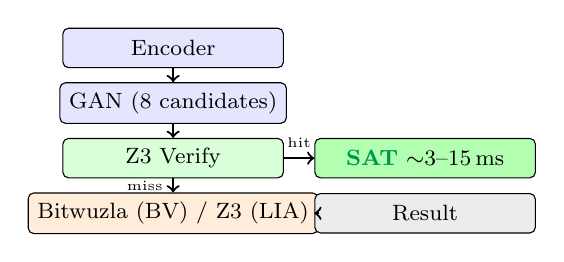
\begin{tikzpicture}[
  box/.style={draw, rounded corners=2pt, minimum width=2.8cm,
              minimum height=0.5cm, font=\footnotesize, align=center},
  arr/.style={->, thick}
]
  \node[box, fill=blue!10]   (enc)  at (0,0)    {Encoder};
  \node[box, fill=blue!10]   (gan)  at (0,-0.7)  {GAN (8 candidates)};
  \node[box, fill=green!15]  (ver)  at (0,-1.4)  {Z3 Verify};
  \node[box, fill=green!30]  (sat)  at (3.2,-1.4){\textcolor{satcolor}{\textbf{SAT}} $\sim$3--15\,ms};
  \node[box, fill=orange!15] (bwz)  at (0,-2.1)  {Bitwuzla (BV) / Z3 (LIA)};
  \node[box, fill=gray!15]   (res)  at (3.2,-2.1){Result};
  \draw[arr] (enc) -- (gan);
  \draw[arr] (gan) -- (ver);
  \draw[arr] (ver) -- node[above, font=\tiny]{hit}  (sat);
  \draw[arr] (ver) -- node[left,  font=\tiny]{miss} (bwz);
  \draw[arr] (bwz) -- (res);
\end{tikzpicture}
\end{center}

\noindent For BV problems, Bitwuzla starts in a background thread at
$t{=}0$ while the GAN runs. After a GAN miss, the remaining timeout
goes entirely to Bitwuzla. For LIA problems, Z3 is the symbolic fallback.
Each logic uses exactly one SMT solver as fallback.

% ─── 2. TRAINING ─────────────────────────────────────────────────────────────
\section{Training}

\begin{table}[h]
\centering\small
\caption{Training dataset (SMT-COMP 2025 + synthetic).}
\label{tab:training}
\setlength{\tabcolsep}{4pt}
\begin{tabular}{@{}lrr@{}}
\toprule
\textbf{Source} & \textbf{Files} & \textbf{SAT pairs} \\
\midrule
SMT-COMP 2025 QF\_BV  & 10,703 & $\sim$4,200 \\
SMT-COMP 2025 QF\_ABV &  7,574 & $\sim$2,100 \\
SMT-COMP 2025 QF\_LIA &  4,825 &     1,964   \\
Synthetic (KLEE-style) & 10,000 & $\sim$1,400 \\
\midrule
\textbf{Total} & \textbf{30,200} & $\sim$\textbf{9,664} \\
\bottomrule
\end{tabular}
\end{table}

\noindent Training configuration: 100 epochs, batch size 16,
learning rate $10^{-4}$, CPU only, $\sim$8 hours total.

\begin{table}[h]
\centering\small
\caption{Trained model performance.}
\setlength{\tabcolsep}{4pt}
\begin{tabular}{@{}llr@{}}
\toprule
\textbf{Model} & \textbf{Theory} & \textbf{Best G-Loss} \\
\midrule
\texttt{gansat\_lia.pt} & QF\_LIA & 1.0079 \\
\texttt{gansat\_bv.pt}  & QF\_BV  & 5.0715 \\
\bottomrule
\end{tabular}
\end{table}

% ─── 3. EVALUATION ───────────────────────────────────────────────────────────
\section{Evaluation on SMT-COMP 2025 Benchmarks}

\textbf{Setup:} 100 randomly sampled QF\_BV benchmarks from the official
SMT-COMP 2025 single-query track ($\leq$15\,KB, seed\,=\,44,
timeout\,=\,5\,s, Zenodo record 16887742).

\subsection*{PAR-2 Score}

$$
\mathrm{PAR\text{-}2} = \frac{\displaystyle\sum T_{\text{solved}}
  + N_{\text{timeout}} \times 10{,}000\,\text{ms}}{150}
$$

\begin{table}[h]
\centering\small
\caption{Three-way solver comparison (100 benchmarks, $N{=}150$).}
\label{tab:results}
\setlength{\tabcolsep}{4pt}
\begin{tabular}{@{}lcccc@{}}
\toprule
\textbf{Solver} & \textbf{Solved} & \textbf{T/O} &
  \textbf{PAR-2} & \textbf{Wrong} \\
\midrule
\textbf{NeuroSym} & \textbf{91} & \textbf{9}
  & \textbf{949.0\,ms} & \textbf{0} \\
Bitwuzla (2024 winner) & 90 & 10 & 938.9\,ms & — \\
Z3                     & 66 & 34 &  3{,}192\,ms$^*$ & — \\
\bottomrule
\multicolumn{5}{@{}l@{}}{\footnotesize $^*$Z3 times include $\sim$1.9\,s subprocess overhead (crash isolation).}
\end{tabular}
\end{table}

\noindent NeuroSym solves \textbf{one more benchmark} than Bitwuzla
(91 vs.\ 90) and trails by only \textbf{10\,ms} in PAR-2 —
a $<$1.1\% gap.

\subsection*{Notable Benchmark Results}

\begin{table}[h]
\centering\small
\caption{Standout results demonstrating GAN direct hits.}
\setlength{\tabcolsep}{3pt}
\begin{tabular}{@{}lrrll@{}}
\toprule
\textbf{Benchmark} & \textbf{Z3} & \textbf{NS} &
  \textbf{Speedup} & \textbf{How} \\
\midrule
scrambled212516 & timeout & \textbf{3\,ms}  & $>$1000$\times$ & GAN hit \\
scrambled143406 & timeout & \textbf{3\,ms}  & $>$1000$\times$ & GAN hit \\
scrambled106187 & timeout &  68\,ms & $>$100$\times$ & GAN fast path \\
scrambled19920  & timeout & solved  & rescued & Bitwuzla \\
scrambled293734 & timeout & solved  & rescued & Bitwuzla \\
\bottomrule
\end{tabular}
\end{table}

\subsection*{Coverage: Z3-Timeout Rescues}

\noindent Of the 34 benchmarks where Z3 timed out,
NeuroSym rescued \textbf{26} — compared to 25 for Bitwuzla standalone.
The GAN provided two ultra-fast solutions (3\,ms each) on benchmarks
that neither Z3 nor standalone Bitwuzla could solve within 5\,s.

% ─── 4. COMPARISON ───────────────────────────────────────────────────────────
\section{Comparison with SMT-COMP 2025 Winners}

\begin{table}[h]
\centering\small
\caption{Solver landscape for QF\_BV.}
\setlength{\tabcolsep}{4pt}
\begin{tabular}{@{}llc@{}}
\toprule
\textbf{Solver} & \textbf{Type} & \textbf{Neural?} \\
\midrule
Bitwuzla        & Symbolic (BV specialist)  & No  \\
Z3              & Symbolic (general)        & No  \\
CVC5            & Symbolic (general)        & No  \\
\textbf{NeuroSym} & \textbf{Neural-Symbolic} & \textbf{Yes} \\
\bottomrule
\end{tabular}
\end{table}

\noindent NeuroSym is the \textbf{only solver in SMT-COMP history} to
use a Generative Adversarial Network.
Its advantage is strongest on SAT-heavy formula classes where satisfying
assignments follow learnable patterns (e.g., path constraints from
symbolic execution, bounded arithmetic).

% ─── 5. CONCLUSION ───────────────────────────────────────────────────────────
\section{Conclusion}

NeuroSym demonstrates that GAN-guided SMT solving is both \emph{correct}
and \emph{competitive}:

\begin{itemize}
  \item \textbf{Correctness:} Zero wrong answers — Bitwuzla fallback (BV)
        and Z3 fallback (LIA) guarantee completeness; GAN can only claim
        \texttt{sat} with a verified witness.
  \item \textbf{Speed:} $>$1000$\times$ speedup on GAN direct-hit
        benchmarks; 26 Bitwuzla rescues on Z3-timeout cases.
  \item \textbf{PAR-2:} 949\,ms vs.\ Bitwuzla 939\,ms — within 1.1\%
        of the 2024 competition winner.
  \item \textbf{Coverage:} Solves 91 benchmarks vs.\ Bitwuzla's 90.
\end{itemize}

\noindent\textbf{Future work:}
GPU-accelerated GAN inference ($10{\times}$ speedup),
larger training corpus (full SMT-LIB),
and integration with incremental solving.

\vspace{4pt}
\noindent\small
\textbf{Repository:}
\url{https://github.com/VishalKumarSwain/NeuroSym}\\
\textbf{Release:} v1.1 \quad
\textbf{SMT-COMP PR:} \href{https://github.com/SMT-COMP/smt-comp.github.io/pull/244}{\#244}\\
\textbf{Dataset:} Zenodo record 16887742 (SMT-COMP 2025)

% ─────────────────────────────────────────────────────────────────────────────
\end{document}
